\documentclass[compress,violet,10pt]{beamer}

\mode<presentation>
\usetheme{Warsaw}

\usepackage{multicol}
\usepackage{amsmath}
\usepackage{hyperref}
\usepackage{graphics} % for including figures
\usepackage{graphicx} % for including figures
\usepackage[update,prepend]{epstopdf} % for including eps in pdf
\def\pdfshellescape{1} % for auto converting eps to pdf
\graphicspath{{../img/}}

\newcommand*\rfrac[2]{{}^{#1}\!/_{#2}}


\useoutertheme[subsection=false]{smoothbars}
\setbeamertemplate{caption}[numbered]
\setbeamercovered{transparent}

\title{Leveraging User's Mood and Song Popularity for Music Recommendation}

\author[Aritra Saha]
{Aritra Saha\\ {\small Supervised by: Dr. Arnab Bhattacharya}}

\institute{Department of Computer Science \& Engineering\\ IIT Kanpur }

\AtBeginSection[]
{
	\frame{\frametitle{Outline}
    \tableofcontents[currentsection]
  }
}

\begin{document}
\frame[plain]{\frametitle{} \titlepage}
\frame{\frametitle{Outline}
  \tableofcontents
}
%===========================================================================
\section{Introduction}
\subsection{}
% -------------------------------------slide--------------------------------
\frame{\frametitle{Motivation}
	\begin{block}{User's Mood}
	\begin{itemize}
	 \item Determined by the features of the recently heard songs
	 \item Usually constant over a short period of time and gradually changes
	\end{itemize}
	\end{block}
\pause
	\begin{block}{Song Popularity}
	\begin{itemize}
		 \item Trending songs as a useful recommendation
		 \item Often overrides user's mood and preference
	\end{itemize}
  \end{block}
}
% -------------------------------------slide--------------------------------
\frame{\frametitle{Contribution of this thesis}
	\begin{block}{Mood Determination}
	\begin{itemize}
	 \item Optimize monitored rolling time duration
	 \item Assigning weights to each contributing feature
	 \item Use of Collaborative Filtering to determine similar users
	\end{itemize}
	\end{block}
\pause
	\begin{block}{Recommendation Tool}
	\begin{itemize}
		 \item Enables customization of weightages
		 \item Recommends songs for a given user
	\end{itemize}
  \end{block}
}
%
%===========================================================================
\section[Background]{Background}
\subsection{}
%-------------------------------------slide---------------------------------
\frame{\frametitle{Related Work}
	\begin{block}{Pandora Radio \& Music Genome}
	\begin{itemize}
		\item Categorzing each song by 300 - 500 genes on a scale of 0-5 with an increment of 0.5, for e.g., Pop/Rock, Jazz, Classical, level of guitar distortion, type of background vocals
		\item Manually analyzed by musicians with 20-30 minutes per song
		\item Vectors are matched by proprietary ``matching algorithm''
	\end{itemize}
  \end{block}
\pause
	\begin{block}{Modelling Internet Radio - Yahoo!}
	\begin{itemize}
		\item Internet Radio, a very close approximation of popular music
		\item Scraping data over time provides a variety of popularity statistics
	\end{itemize}
	\end{block}
}
%-------------------------------------slide---------------------------------
\frame{\frametitle{Data Structures \& Algorithms}
  \begin{beamerboxesrounded}[shadow=true]{}
	\begin{itemize}
		\item Trie: A tree structure for prefix matching, used mostly for dictionary storage
		\item Levenshtein Distance: Measure distance between 2 strings with a score for addition, deletion \& substitution
		\item Hungarian Algorithm: Optimal assignment for a given cost matrix
		\item Cosine Similarity: Given 2 vectors, a measure of similarity, ranges from -1 to 1
	\end{itemize}
  \end{beamerboxesrounded}
}
%-------------------------------------slide---------------------------------
\frame{\frametitle{Data Acquisition}
	\begin{block}{Million Song Dataset}
	\begin{itemize}
		\item Compiled music data from multiple sources, for e.g., EchoNest, MusicBrainz, SecondHandSongs, Last.FM
		\item Has metadata as well as MFCC features with a disk occupancy of 250GB
		\item Cross-referenced tags from other music data websites for other information
	\end{itemize}
  \end{block}
\pause
	\begin{block}{Last.FM}
	\begin{itemize}
		\item Fetch user's recent history, build up local database for collaborative filtering
		\item Get song's genre information to profile users' based on musical taste
	\end{itemize}
	\end{block}
}

%===========================================================================
\section[Recommendation]{Recommendation}
\subsection{}

%-------------------------------------slide---------------------------------
\frame{\frametitle{Loading Data}
	\begin{block}{Load Million Song}
	\begin{itemize}
		\item Million songs' commonly required information, for e.g., title \& artist loaded up in a trie
		\item Song titles as the keys, enables faster searching while cleaning up user history data
		\item Further information of the songs are loaded into memory on demand to be used while recommending
	\end{itemize}
  \end{block}
\pause
	\begin{block}{User History}
	\begin{itemize}
		\item 2,614 users' recent history has been compiled from Last.FM
		\item History has been cleaned up against the million songs
	\end{itemize}
	\end{block}
}

%-------------------------------------slide---------------------------------
\frame{\frametitle{Profiling}
	\begin{block}{Collaborative Filtering}
	\begin{itemize}
		\item Based on the genres of the songs history, a normalized genre vector is populated which denotes the user's musical taste
		\item A set of 127 commonly found genres are considered for categorzing
		\item Cosine similarity mesaures the similarity between any 2 users
		\item Top \emph{k} users' history are to be considered while recommending for a current user
	\end{itemize}
  \end{block}
\pause
	\begin{block}{Mood Determination}
	\begin{itemize}
		\item Any \emph{m} consecutive songs in a given history defines the mood at point in time
		\item A rolling window of \emph{m} tracks is used to search for a similar mood in the top \emph{k} similar users as that of the current user's present mood
		\item Given 2 mood windows, Hungarian algorithm determines the similarity score
	\end{itemize}
	\end{block}
}

%-------------------------------------slide---------------------------------
 \frame{\frametitle{Song Features \& Comparison}
   \begin{beamerboxesrounded}[shadow=true]{}
 	\begin{itemize}
 	 \item Artist: 2 artists are compared in a similar way users are compared, by the use of consine similarity on their genre vectors
 	 \item Loudness: Logarithm of maximum power represented by the song. Ranges -100 to 100 dB
 	 \item Tempo: Average beats per minute. Determines the pace of the song. Ranges 0 to 500
 	 \item Popularity: Data provided as of 2010. Ranges 0 to 1
 	\end{itemize}
   \end{beamerboxesrounded}
}
%-------------------------------------slide---------------------------------
\frame{\frametitle{Work Flow}
     \begin{figure}
	\centering
	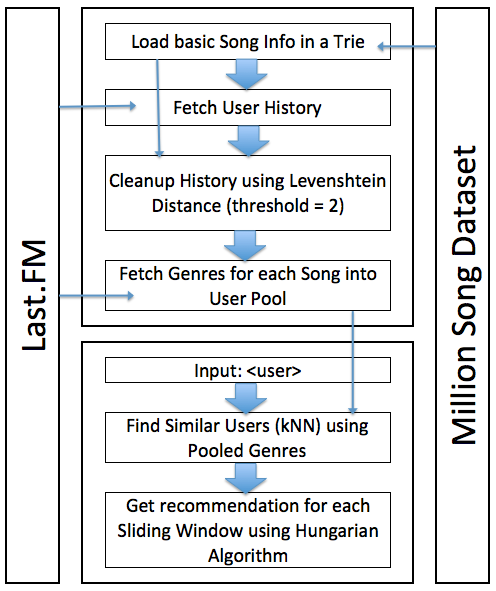
\includegraphics[scale=0.3]{../img/work_flow}
	\caption{Work Flow}
	\label{fig:workflow}
    \end{figure}
}
%===========================================================================
\section[Performance Evaluation and Future Work]{Performance Evaluation and Future Work}
\subsection{}

%-------------------------------------slide---------------------------------
\frame{\frametitle{Weightages}
	\begin{block}{Song Features}
	\begin{itemize}
		\item Artist similarity has been assigned a weight of 60\%
		\item 20\% each for loudness \& tempo
		\item These values have been evaluated to good results
	\end{itemize}
  \end{block}
\pause
	\begin{block}{Similarity v/s Popularity}
	\begin{itemize}
		\item 65\% weightage has been assgined to similarity and 35\% to popularity
		\item A few number of test runs suggested the above weightages to be good
	\end{itemize}
	\end{block}
}
%-------------------------------------slide---------------------------------
\frame{\frametitle{Performance Evaluation}
  \begin{beamerboxesrounded}[shadow=true]{}
	\begin{itemize}
		 \item Most recent \emph{t} tracks have been considered for testing
		 \item Following \emph{m} tracks are taken for current mood
		 \item Recommended songs are then matched with the \emph{t} tracks
		 \item The rank of the top recommendation that appears in the test set is noted
		 \item The similarity of the most similar mood window is also noted
	\end{itemize}
  \end{beamerboxesrounded}
}
%-------------------------------------slide---------------------------------
\frame{\frametitle{Test Run 1}
  \begin{beamerboxesrounded}[shadow=true]{}
    \begin{table}[h!]
\centering
\begin{tabular}{ | c | c | c || c | c | }
\hline
Similar Users	& Mood Length	& Weights							&Confidence	&Rank\\
\hline \hline
50			& 5			& \(\rfrac{1}{3}, \rfrac{1}{3}, \rfrac{1}{3}\)	&62.89 \%		&944\\
\hline
75			& 5			& \(\rfrac{1}{3}, \rfrac{1}{3}, \rfrac{1}{3}\)	&48.45 \%		&3879\\
\hline
100			& 5			& \(\rfrac{1}{3}, \rfrac{1}{3}, \rfrac{1}{3}\)	&48.45 \%		&84\\
\hline
150			& 5			& \(\rfrac{1}{3}, \rfrac{1}{3}, \rfrac{1}{3}\)	&51.01 \%		&135\\
\hline
200			& 5			& \(\rfrac{1}{3}, \rfrac{1}{3}, \rfrac{1}{3}\)	&52.63 \%		&211\\
\hline
50			& 10			& \(\rfrac{1}{3}, \rfrac{1}{3}, \rfrac{1}{3}\)	&45.06 \%		&3418\\
\hline
75			& 10			& \(\rfrac{1}{3}, \rfrac{1}{3}, \rfrac{1}{3}\)	&45.50 \%		&4751\\
\hline
100			& 10			& \(\rfrac{1}{3}, \rfrac{1}{3}, \rfrac{1}{3}\)	&46.93 \%		&1722\\
\hline
50			& 5			& \(\rfrac{1}{5}, \rfrac{2}{5}, \rfrac{2}{5}\)	&43.28 \%		&4033\\
\hline
50			& 5			& \(\rfrac{3}{5}, \rfrac{1}{5}, \rfrac{1}{5}\)	&70.57 \%		&936\\
\hline
75			& 5			& \(\rfrac{3}{5}, \rfrac{1}{5}, \rfrac{1}{5}\)	&60.03 \%		&4367\\
\hline
100			& 5			& \(\rfrac{3}{5}, \rfrac{1}{5}, \rfrac{1}{5}\)	&62.10 \%		&78\\
\hline
150			& 5			& \(\rfrac{3}{5}, \rfrac{1}{5}, \rfrac{1}{5}\)	&64.73 \%		&120\\
\hline
\end{tabular}
\caption{Test Results for Last.FM user: \emph{3en}}
\label{table:test_results_3en}
\end{table}
  \end{beamerboxesrounded}
}
%-------------------------------------slide---------------------------------
\frame{\frametitle{Test Run 2}
  \begin{beamerboxesrounded}[shadow=true]{}
   \begin{table}[h!]
\centering
\begin{tabular}{ | c | c | c || c | c | }
\hline
Similar Users	& Mood Length	& Weights							&Confidence	&Rank\\
\hline \hline
50			& 5			& \(\rfrac{1}{3}, \rfrac{1}{3}, \rfrac{1}{3}\)	&62.39 \%		&2376\\
\hline
75			& 5			& \(\rfrac{1}{3}, \rfrac{1}{3}, \rfrac{1}{3}\)	&50.43 \%		&N/A\\
\hline
100			& 5			& \(\rfrac{1}{3}, \rfrac{1}{3}, \rfrac{1}{3}\)	&50.43 \%		&7608\\
\hline
150			& 5			& \(\rfrac{1}{3}, \rfrac{1}{3}, \rfrac{1}{3}\)	&50.43 \%		&8828\\
\hline
200			& 5			& \(\rfrac{1}{3}, \rfrac{1}{3}, \rfrac{1}{3}\)	&52.40 \%		&10018\\
\hline
50			& 10			& \(\rfrac{1}{3}, \rfrac{1}{3}, \rfrac{1}{3}\)	&48.91 \%		&N/A\\
\hline
75			& 10			& \(\rfrac{1}{3}, \rfrac{1}{3}, \rfrac{1}{3}\)	&48.91 \%		&N/A\\
\hline
100			& 10			& \(\rfrac{1}{3}, \rfrac{1}{3}, \rfrac{1}{3}\)	&48.91 \%		&N/A\\
\hline
50			& 5			& \(\rfrac{1}{5}, \rfrac{2}{5}, \rfrac{2}{5}\)	&43.28 \%		&N/A\\
\hline
50			& 5			& \(\rfrac{3}{5}, \rfrac{1}{5}, \rfrac{1}{5}\)	&70.70 \%		&2391\\
\hline
75			& 5			& \(\rfrac{3}{5}, \rfrac{1}{5}, \rfrac{1}{5}\)	&66.15 \%		&N/A\\
\hline
100			& 5			& \(\rfrac{3}{5}, \rfrac{1}{5}, \rfrac{1}{5}\)	&66.15 \%		&7095\\
\hline
150			& 5			& \(\rfrac{3}{5}, \rfrac{1}{5}, \rfrac{1}{5}\)	&66.15 \%		&7767\\
\hline
\end{tabular}
\caption{Test Results for Last.FM user: \emph{RJ}}
\label{table:test_results_rj}
\end{table}
  \end{beamerboxesrounded}
}
%-------------------------------------slide---------------------------------
\frame{\frametitle{Test Run 3}
  \begin{beamerboxesrounded}[shadow=true]{}
  \begin{table}[h!]
\centering
\begin{tabular}{ | c | c | c || c | c | }
\hline
Similar Users	& Mood Length	& Weights							&Confidence	&Rank\\
\hline \hline
50			& 5			& \(\rfrac{1}{3}, \rfrac{1}{3}, \rfrac{1}{3}\)	&62.59 \%		&59\\
\hline
75			& 5			& \(\rfrac{1}{3}, \rfrac{1}{3}, \rfrac{1}{3}\)	&50.43 \%		&607\\
\hline
100			& 5			& \(\rfrac{1}{3}, \rfrac{1}{3}, \rfrac{1}{3}\)	&48.37 \%		&736\\
\hline
150			& 5			& \(\rfrac{1}{3}, \rfrac{1}{3}, \rfrac{1}{3}\)	&51.94 \%		&1095\\
\hline
200			& 5			& \(\rfrac{1}{3}, \rfrac{1}{3}, \rfrac{1}{3}\)	&51.94 \%		&1428\\
\hline
50			& 10			& \(\rfrac{1}{3}, \rfrac{1}{3}, \rfrac{1}{3}\)	&48.91 \%		&2632\\
\hline
75			& 10			& \(\rfrac{1}{3}, \rfrac{1}{3}, \rfrac{1}{3}\)	&48.91 \%		&3736\\
\hline
100			& 10			& \(\rfrac{1}{3}, \rfrac{1}{3}, \rfrac{1}{3}\)	&46.91 \%		&4304\\
\hline
50			& 5			& \(\rfrac{1}{5}, \rfrac{2}{5}, \rfrac{2}{5}\)	&43.28 \%		&563\\
\hline
50			& 5			& \(\rfrac{3}{5}, \rfrac{1}{5}, \rfrac{1}{5}\)	&70.94 \%		&85\\
\hline
75			& 5			& \(\rfrac{3}{5}, \rfrac{1}{5}, \rfrac{1}{5}\)	&66.15 \%		&555\\
\hline
100			& 5			& \(\rfrac{3}{5}, \rfrac{1}{5}, \rfrac{1}{5}\)	&63.88 \%		&650\\
\hline
150			& 5			& \(\rfrac{3}{5}, \rfrac{1}{5}, \rfrac{1}{5}\)	&64.59 \%		&970\\
\hline
\end{tabular}
\caption{Test Results for Last.FM user: \emph{eartle}}
\label{table:test_results_eartle}
\end{table}
  \end{beamerboxesrounded}
}
%-------------------------------------slide---------------------------------
\frame{\frametitle{Test Run 4}
  \begin{beamerboxesrounded}[shadow=true]{}
  \begin{table}[h!]
\centering
\begin{tabular}{ | c | c | c || c | c | }
\hline
Similar Users	& Mood Length	& Weights							&Confidence	&Rank\\
\hline \hline
50			& 5			& \(\rfrac{1}{3}, \rfrac{1}{3}, \rfrac{1}{3}\)	&61.84 \%		&141\\
\hline
75			& 5			& \(\rfrac{1}{3}, \rfrac{1}{3}, \rfrac{1}{3}\)	&49.83 \%		&629\\
\hline
100			& 5			& \(\rfrac{1}{3}, \rfrac{1}{3}, \rfrac{1}{3}\)	&49.71 \%		&674\\
\hline
150			& 5			& \(\rfrac{1}{3}, \rfrac{1}{3}, \rfrac{1}{3}\)	&51.10 \%		&4351\\
\hline
200			& 5			& \(\rfrac{1}{3}, \rfrac{1}{3}, \rfrac{1}{3}\)	&51.48 \%		&4363\\
\hline
50			& 10			& \(\rfrac{1}{3}, \rfrac{1}{3}, \rfrac{1}{3}\)	&47.49 \%		&3160\\
\hline
75			& 10			& \(\rfrac{1}{3}, \rfrac{1}{3}, \rfrac{1}{3}\)	&47.49 \%		&3135\\
\hline
100			& 10			& \(\rfrac{1}{3}, \rfrac{1}{3}, \rfrac{1}{3}\)	&47.54 \%		&3225\\
\hline
50			& 5			& \(\rfrac{1}{5}, \rfrac{2}{5}, \rfrac{2}{5}\)	&43.28 \%		&4422\\
\hline
50			& 5			& \(\rfrac{3}{5}, \rfrac{1}{5}, \rfrac{1}{5}\)	&67.74 \%		&103\\
\hline
75			& 5			& \(\rfrac{3}{5}, \rfrac{1}{5}, \rfrac{1}{5}\)	&66.18 \%		&470\\
\hline
100			& 5			& \(\rfrac{3}{5}, \rfrac{1}{5}, \rfrac{1}{5}\)	&64.43 \%		&471\\
\hline
150			& 5			& \(\rfrac{3}{5}, \rfrac{1}{5}, \rfrac{1}{5}\)	&64.43 \%		&5227\\
\hline
\end{tabular}
\caption{Test Results for Last.FM user: \emph{franhale}}
\label{table:test_results_franhale}
\end{table}
  \end{beamerboxesrounded}
}
%-------------------------------------slide---------------------------------
\frame{\frametitle{Test Run 5}
  \begin{beamerboxesrounded}[shadow=true]{}
  \begin{table}[h!]
\centering
\begin{tabular}{ | c | c | c || c | c | }
\hline
Similar Users	& Mood Length	& Weights							&Confidence	&Rank\\
\hline \hline
50			& 5			& \(\rfrac{1}{3}, \rfrac{1}{3}, \rfrac{1}{3}\)	&62.64 \%		&4953\\
\hline
75			& 5			& \(\rfrac{1}{3}, \rfrac{1}{3}, \rfrac{1}{3}\)	&50.09 \%		&9857\\
\hline
100			& 5			& \(\rfrac{1}{3}, \rfrac{1}{3}, \rfrac{1}{3}\)	&50.09 \%		&11647\\
\hline
150			& 5			& \(\rfrac{1}{3}, \rfrac{1}{3}, \rfrac{1}{3}\)	&51.10 \%		&6587\\
\hline
200			& 5			& \(\rfrac{1}{3}, \rfrac{1}{3}, \rfrac{1}{3}\)	&51.48 \%		&8008\\
\hline
50			& 10			& \(\rfrac{1}{3}, \rfrac{1}{3}, \rfrac{1}{3}\)	&48.08 \%		&N/A\\
\hline
75			& 10			& \(\rfrac{1}{3}, \rfrac{1}{3}, \rfrac{1}{3}\)	&48.08 \%		&2584\\
\hline
100			& 10			& \(\rfrac{1}{3}, \rfrac{1}{3}, \rfrac{1}{3}\)	&48.08 \%		&2887\\
\hline
50			& 5			& \(\rfrac{1}{5}, \rfrac{2}{5}, \rfrac{2}{5}\)	&43.28 \%		&N/A\\
\hline
50			& 5			& \(\rfrac{3}{5}, \rfrac{1}{5}, \rfrac{1}{5}\)	&70.75 \%		&5005\\
\hline
75			& 5			& \(\rfrac{3}{5}, \rfrac{1}{5}, \rfrac{1}{5}\)	&65.97 \%		&7819\\
\hline
100			& 5			& \(\rfrac{3}{5}, \rfrac{1}{5}, \rfrac{1}{5}\)	&65.97 \%		&9345\\
\hline
150			& 5			& \(\rfrac{3}{5}, \rfrac{1}{5}, \rfrac{1}{5}\)	&68.19 \%		&5749\\
\hline
\end{tabular}
\caption{Test Results for Last.FM user: \emph{massdosage}}
\label{table:test_results_massdosage}
\end{table}
  \end{beamerboxesrounded}
}
%-------------------------------------slide---------------------------------
\frame{\frametitle{Optimizations}
  \begin{beamerboxesrounded}[shadow=true]{}
     \begin{itemize}
      \item Parallelization: Independent jobs have been forked in parallel to reduce runtime
      \item On-Demand Caching: Not only avoids loading the entire DB into memory, but also prevents disk access each time the same resource is called for. Also reduces multiple file accesses
      \item Minimal data handling: Minimal data is stored in memory in a serialized JSON format
     \end{itemize}
  \end{beamerboxesrounded}
}
%-------------------------------------slide---------------------------------
\frame{\frametitle{Future Work}
  \begin{beamerboxesrounded}[shadow=true]{}
	\begin{itemize}
		 \item Larger and newer dataset
		 \item Machine learning to implement feedback mechanism for user specific weightages
		 \item More features like MFCC can be included appropriately
		 \item Code can be optimized even further by the use of distributed systems
	\end{itemize}
  \end{beamerboxesrounded}
}

%-------------------------------------slide---------------------------------
\frame{\frametitle{}
%  \begin{beamerboxesrounded}[shadow=true]{}
   %\centering{\Large{Questions?}}
    \begin{figure}
      \centering
      
\includegraphics[scale=0.2]{../img/questions.png}
    \end{figure}
%  \end{beamerboxesrounded}
}

%-------------------------------------slide---------------------------------
\frame{\frametitle{}
  \begin{beamerboxesrounded}[shadow=true]{}
   \centering{\Large{Thank you!}}
  \end{beamerboxesrounded}
}
\end{document}
